\documentclass[twoside]{book}

% Packages required by doxygen
\usepackage{fixltx2e}
\usepackage{calc}
\usepackage{doxygen}
\usepackage[export]{adjustbox} % also loads graphicx
\usepackage{graphicx}
\usepackage[utf8]{inputenc}
\usepackage{makeidx}
\usepackage{multicol}
\usepackage{multirow}
\PassOptionsToPackage{warn}{textcomp}
\usepackage{textcomp}
\usepackage[nointegrals]{wasysym}
\usepackage[table]{xcolor}

% NLS support packages
\usepackage[spanish]{babel}
% Font selection
\usepackage[T1]{fontenc}
\usepackage[scaled=.90]{helvet}
\usepackage{courier}
\usepackage{amssymb}
\usepackage{sectsty}
\renewcommand{\familydefault}{\sfdefault}
\allsectionsfont{%
  \fontseries{bc}\selectfont%
  \color{darkgray}%
}
\renewcommand{\DoxyLabelFont}{%
  \fontseries{bc}\selectfont%
  \color{darkgray}%
}
\newcommand{\+}{\discretionary{\mbox{\scriptsize$\hookleftarrow$}}{}{}}

% Page & text layout
\usepackage{geometry}
\geometry{%
  a4paper,%
  top=2.5cm,%
  bottom=2.5cm,%
  left=2.5cm,%
  right=2.5cm%
}
\tolerance=750
\hfuzz=15pt
\hbadness=750
\setlength{\emergencystretch}{15pt}
\setlength{\parindent}{0cm}
\setlength{\parskip}{3ex plus 2ex minus 2ex}
\makeatletter
\renewcommand{\paragraph}{%
  \@startsection{paragraph}{4}{0ex}{-1.0ex}{1.0ex}{%
    \normalfont\normalsize\bfseries\SS@parafont%
  }%
}
\renewcommand{\subparagraph}{%
  \@startsection{subparagraph}{5}{0ex}{-1.0ex}{1.0ex}{%
    \normalfont\normalsize\bfseries\SS@subparafont%
  }%
}
\makeatother

% Headers & footers
\usepackage{fancyhdr}
\pagestyle{fancyplain}
\fancyhead[LE]{\fancyplain{}{\bfseries\thepage}}
\fancyhead[CE]{\fancyplain{}{}}
\fancyhead[RE]{\fancyplain{}{\bfseries\leftmark}}
\fancyhead[LO]{\fancyplain{}{\bfseries\rightmark}}
\fancyhead[CO]{\fancyplain{}{}}
\fancyhead[RO]{\fancyplain{}{\bfseries\thepage}}
\fancyfoot[LE]{\fancyplain{}{}}
\fancyfoot[CE]{\fancyplain{}{}}
\fancyfoot[RE]{\fancyplain{}{\bfseries\scriptsize Generado por Doxygen }}
\fancyfoot[LO]{\fancyplain{}{\bfseries\scriptsize Generado por Doxygen }}
\fancyfoot[CO]{\fancyplain{}{}}
\fancyfoot[RO]{\fancyplain{}{}}
\renewcommand{\footrulewidth}{0.4pt}
\renewcommand{\chaptermark}[1]{%
  \markboth{#1}{}%
}
\renewcommand{\sectionmark}[1]{%
  \markright{\thesection\ #1}%
}

% Indices & bibliography
\usepackage{natbib}
\usepackage[titles]{tocloft}
\setcounter{tocdepth}{3}
\setcounter{secnumdepth}{5}
\makeindex

% Hyperlinks (required, but should be loaded last)
\usepackage{ifpdf}
\ifpdf
  \usepackage[pdftex,pagebackref=true]{hyperref}
\else
  \usepackage[ps2pdf,pagebackref=true]{hyperref}
\fi
\hypersetup{%
  colorlinks=true,%
  linkcolor=blue,%
  citecolor=blue,%
  unicode%
}

% Custom commands
\newcommand{\clearemptydoublepage}{%
  \newpage{\pagestyle{empty}\cleardoublepage}%
}

\usepackage{caption}
\captionsetup{labelsep=space,justification=centering,font={bf},singlelinecheck=off,skip=4pt,position=top}

%===== C O N T E N T S =====

\begin{document}

% Titlepage & ToC
\hypersetup{pageanchor=false,
             bookmarksnumbered=true,
             pdfencoding=unicode
            }
\pagenumbering{roman}
\begin{titlepage}
\vspace*{7cm}
\begin{center}%
{\Large Rm\+Lib \\[1ex]\large 1.\+0.\+0v }\\
\vspace*{1cm}
{\large Generado por Doxygen 1.8.11}\\
\end{center}
\end{titlepage}
\clearemptydoublepage
\tableofcontents
\clearemptydoublepage
\pagenumbering{arabic}
\hypersetup{pageanchor=true}

%--- Begin generated contents ---
\chapter{Indice jerárquico}
\section{Jerarquía de la clase}
Esta lista de herencias esta ordenada aproximadamente por orden alfabético\+:\begin{DoxyCompactList}
\item Q\+Main\+Window\begin{DoxyCompactList}
\item \contentsline{section}{Main\+Window}{\pageref{classMainWindow}}{}
\end{DoxyCompactList}
\item Q\+Object\begin{DoxyCompactList}
\item \contentsline{section}{Socket\+Cliente}{\pageref{classSocketCliente}}{}
\end{DoxyCompactList}
\end{DoxyCompactList}

\chapter{Índice de clases}
\section{Lista de clases}
Lista de las clases, estructuras, uniones e interfaces con una breve descripción\+:\begin{DoxyCompactList}
\item\contentsline{section}{\hyperlink{classMainWindow}{Main\+Window} \\*The \hyperlink{classMainWindow}{Main\+Window} class }{\pageref{classMainWindow}}{}
\item\contentsline{section}{\hyperlink{classSocketCliente}{Socket\+Cliente} \\*The \hyperlink{classSocketCliente}{Socket\+Cliente} class }{\pageref{classSocketCliente}}{}
\end{DoxyCompactList}

\chapter{Indice de archivos}
\section{Lista de archivos}
Lista de todos los archivos documentados y con descripciones breves\+:\begin{DoxyCompactList}
\item\contentsline{section}{\hyperlink{mainwindow_8h}{mainwindow.\+h} \\*\hyperlink{classMainWindow}{Main\+Window} header }{\pageref{mainwindow_8h}}{}
\item\contentsline{section}{\hyperlink{socketcliente_8h}{socketcliente.\+h} \\*Contains a set of methods for handling Socket connection }{\pageref{socketcliente_8h}}{}
\end{DoxyCompactList}

\chapter{Documentación de las clases}
\hypertarget{classMainWindow}{}\section{Referencia de la Clase Main\+Window}
\label{classMainWindow}\index{Main\+Window@{Main\+Window}}


The \hyperlink{classMainWindow}{Main\+Window} class.  




{\ttfamily \#include $<$mainwindow.\+h$>$}



Diagrama de herencias de Main\+Window
\nopagebreak
\begin{figure}[H]
\begin{center}
\leavevmode
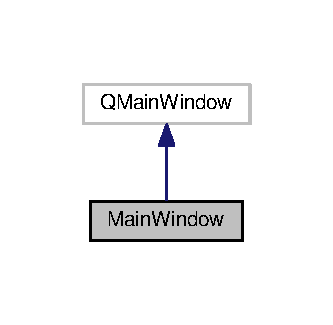
\includegraphics[width=160pt]{classMainWindow__inherit__graph}
\end{center}
\end{figure}


Diagrama de colaboración para Main\+Window\+:
\nopagebreak
\begin{figure}[H]
\begin{center}
\leavevmode
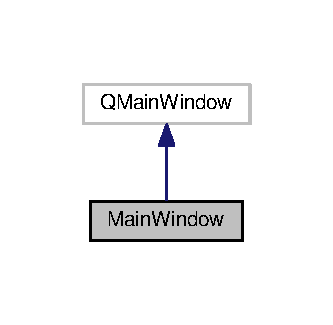
\includegraphics[width=160pt]{classMainWindow__coll__graph}
\end{center}
\end{figure}
\subsection*{Métodos públicos}
\begin{DoxyCompactItemize}
\item 
\hyperlink{classMainWindow_a8b244be8b7b7db1b08de2a2acb9409db}{Main\+Window} (Q\+Widget $\ast$parent=0)
\begin{DoxyCompactList}\small\item\em Constructor. \end{DoxyCompactList}\item 
\hyperlink{classMainWindow_ae98d00a93bc118200eeef9f9bba1dba7}{$\sim$\+Main\+Window} ()\hypertarget{classMainWindow_ae98d00a93bc118200eeef9f9bba1dba7}{}\label{classMainWindow_ae98d00a93bc118200eeef9f9bba1dba7}

\begin{DoxyCompactList}\small\item\em Destructor. \end{DoxyCompactList}\end{DoxyCompactItemize}


\subsection{Descripción detallada}
The \hyperlink{classMainWindow}{Main\+Window} class. 

\subsection{Documentación del constructor y destructor}
\index{Main\+Window@{Main\+Window}!Main\+Window@{Main\+Window}}
\index{Main\+Window@{Main\+Window}!Main\+Window@{Main\+Window}}
\subsubsection[{\texorpdfstring{Main\+Window(\+Q\+Widget $\ast$parent=0)}{MainWindow(QWidget *parent=0)}}]{\setlength{\rightskip}{0pt plus 5cm}Main\+Window\+::\+Main\+Window (
\begin{DoxyParamCaption}
\item[{Q\+Widget $\ast$}]{parent = {\ttfamily 0}}
\end{DoxyParamCaption}
)\hspace{0.3cm}{\ttfamily [explicit]}}\hypertarget{classMainWindow_a8b244be8b7b7db1b08de2a2acb9409db}{}\label{classMainWindow_a8b244be8b7b7db1b08de2a2acb9409db}


Constructor. 


\begin{DoxyParams}{Parámetros}
{\em parent} & -\/ pointer of Q\+Widget object. \\
\hline
\end{DoxyParams}


La documentación para esta clase fue generada a partir de los siguientes ficheros\+:\begin{DoxyCompactItemize}
\item 
\hyperlink{mainwindow_8h}{mainwindow.\+h}\item 
mainwindow.\+cpp\end{DoxyCompactItemize}

\hypertarget{classSocketCliente}{}\section{Referencia de la Clase Socket\+Cliente}
\label{classSocketCliente}\index{Socket\+Cliente@{Socket\+Cliente}}


The \hyperlink{classSocketCliente}{Socket\+Cliente} class.  




{\ttfamily \#include $<$socketcliente.\+h$>$}



Diagrama de herencias de Socket\+Cliente
\nopagebreak
\begin{figure}[H]
\begin{center}
\leavevmode
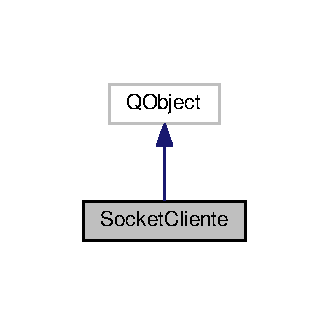
\includegraphics[width=158pt]{classSocketCliente__inherit__graph}
\end{center}
\end{figure}


Diagrama de colaboración para Socket\+Cliente\+:
\nopagebreak
\begin{figure}[H]
\begin{center}
\leavevmode
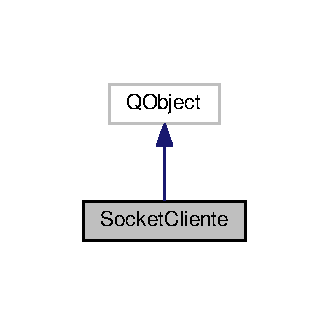
\includegraphics[width=158pt]{classSocketCliente__coll__graph}
\end{center}
\end{figure}
\subsection*{Señales}
\begin{DoxyCompactItemize}
\item 
void \hyperlink{classSocketCliente_a5203829ebf869208e859c7a9306b5985}{new\+\_\+msg} (Q\+String msj)
\begin{DoxyCompactList}\small\item\em Signal when a new message is recived. \end{DoxyCompactList}\end{DoxyCompactItemize}
\subsection*{Métodos públicos}
\begin{DoxyCompactItemize}
\item 
\hyperlink{classSocketCliente_aad9035a6cc6339a73bc1683357ad5260}{Socket\+Cliente} (int portA, int portB, string ipA, string ipB)\hypertarget{classSocketCliente_aad9035a6cc6339a73bc1683357ad5260}{}\label{classSocketCliente_aad9035a6cc6339a73bc1683357ad5260}

\begin{DoxyCompactList}\small\item\em Constructor. \end{DoxyCompactList}\item 
\hyperlink{classSocketCliente_a824901a5f9a1255960fc0ffcc10be678}{$\sim$\+Socket\+Cliente} ()\hypertarget{classSocketCliente_a824901a5f9a1255960fc0ffcc10be678}{}\label{classSocketCliente_a824901a5f9a1255960fc0ffcc10be678}

\begin{DoxyCompactList}\small\item\em Destructor. \end{DoxyCompactList}\item 
bool \hyperlink{classSocketCliente_a61f809a0f5f4f3aeca6f3114056183f8}{connect\+\_\+socket} ()
\begin{DoxyCompactList}\small\item\em Connect the Socket\+Client with Server. \end{DoxyCompactList}\item 
void \hyperlink{classSocketCliente_ae041582d856886a8e0a168a26aab27bd}{set\+\_\+msj} (const char $\ast$msj)
\begin{DoxyCompactList}\small\item\em Send messages to Server. \end{DoxyCompactList}\end{DoxyCompactItemize}


\subsection{Descripción detallada}
The \hyperlink{classSocketCliente}{Socket\+Cliente} class. 

\subsection{Documentación de las funciones miembro}
\index{Socket\+Cliente@{Socket\+Cliente}!connect\+\_\+socket@{connect\+\_\+socket}}
\index{connect\+\_\+socket@{connect\+\_\+socket}!Socket\+Cliente@{Socket\+Cliente}}
\subsubsection[{\texorpdfstring{connect\+\_\+socket()}{connect_socket()}}]{\setlength{\rightskip}{0pt plus 5cm}bool Socket\+Cliente\+::connect\+\_\+socket (
\begin{DoxyParamCaption}
{}
\end{DoxyParamCaption}
)}\hypertarget{classSocketCliente_a61f809a0f5f4f3aeca6f3114056183f8}{}\label{classSocketCliente_a61f809a0f5f4f3aeca6f3114056183f8}


Connect the Socket\+Client with Server. 

\begin{DoxyReturn}{Devuelve}

\end{DoxyReturn}
\index{Socket\+Cliente@{Socket\+Cliente}!new\+\_\+msg@{new\+\_\+msg}}
\index{new\+\_\+msg@{new\+\_\+msg}!Socket\+Cliente@{Socket\+Cliente}}
\subsubsection[{\texorpdfstring{new\+\_\+msg}{new_msg}}]{\setlength{\rightskip}{0pt plus 5cm}void Socket\+Cliente\+::new\+\_\+msg (
\begin{DoxyParamCaption}
\item[{Q\+String}]{msj}
\end{DoxyParamCaption}
)\hspace{0.3cm}{\ttfamily [signal]}}\hypertarget{classSocketCliente_a5203829ebf869208e859c7a9306b5985}{}\label{classSocketCliente_a5203829ebf869208e859c7a9306b5985}


Signal when a new message is recived. 


\begin{DoxyParams}{Parámetros}
{\em msj} & -\/ recived message. \\
\hline
\end{DoxyParams}
\index{Socket\+Cliente@{Socket\+Cliente}!set\+\_\+msj@{set\+\_\+msj}}
\index{set\+\_\+msj@{set\+\_\+msj}!Socket\+Cliente@{Socket\+Cliente}}
\subsubsection[{\texorpdfstring{set\+\_\+msj(const char $\ast$msj)}{set_msj(const char *msj)}}]{\setlength{\rightskip}{0pt plus 5cm}void Socket\+Cliente\+::set\+\_\+msj (
\begin{DoxyParamCaption}
\item[{const char $\ast$}]{msj}
\end{DoxyParamCaption}
)}\hypertarget{classSocketCliente_ae041582d856886a8e0a168a26aab27bd}{}\label{classSocketCliente_ae041582d856886a8e0a168a26aab27bd}


Send messages to Server. 


\begin{DoxyParams}{Parámetros}
{\em msj} & -\/ message to send. \\
\hline
\end{DoxyParams}


La documentación para esta clase fue generada a partir de los siguientes ficheros\+:\begin{DoxyCompactItemize}
\item 
\hyperlink{socketcliente_8h}{socketcliente.\+h}\item 
socketcliente.\+cpp\end{DoxyCompactItemize}

\chapter{Documentación de archivos}
\hypertarget{mainwindow_8h}{}\section{mainwindow.\+h File Reference}
\label{mainwindow_8h}\index{mainwindow.\+h@{mainwindow.\+h}}


\hyperlink{classMainWindow}{Main\+Window} header.  


{\ttfamily \#include $<$Q\+Main\+Window$>$}\\*
{\ttfamily \#include $<$Q\+Message\+Box$>$}\\*
{\ttfamily \#include \char`\"{}socketserver.\+h\char`\"{}}\\*
Include dependency graph for mainwindow.\+h\+:
\nopagebreak
\begin{figure}[H]
\begin{center}
\leavevmode
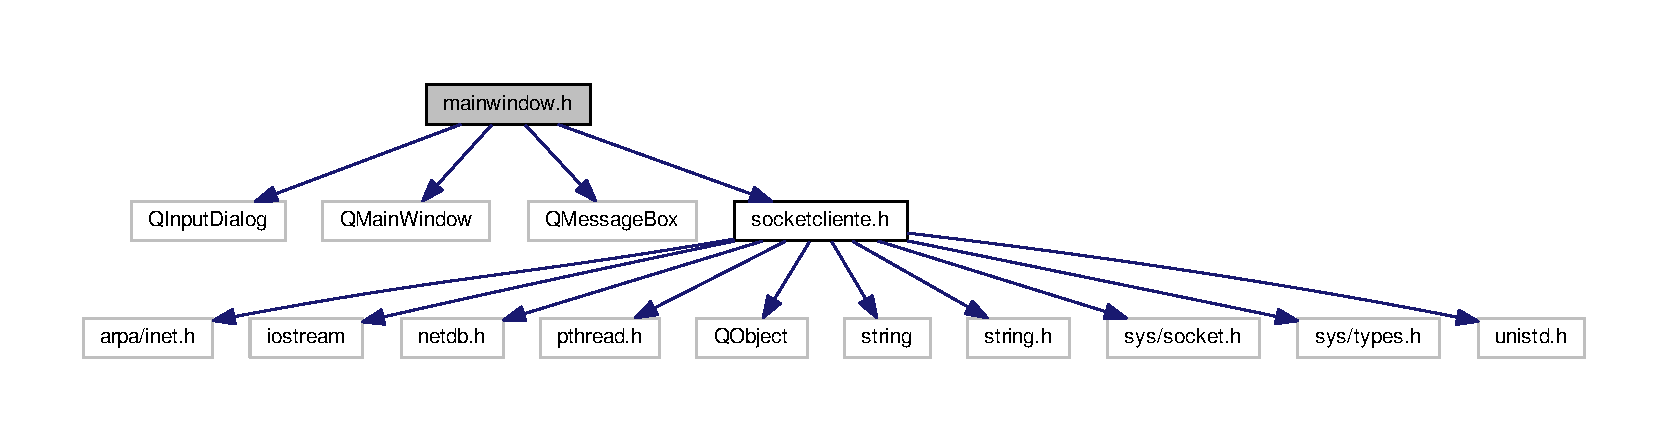
\includegraphics[width=350pt]{mainwindow_8h__incl}
\end{center}
\end{figure}
\subsection*{Classes}
\begin{DoxyCompactItemize}
\item 
class \hyperlink{classMainWindow}{Main\+Window}
\begin{DoxyCompactList}\small\item\em The \hyperlink{classMainWindow}{Main\+Window} class. \end{DoxyCompactList}\end{DoxyCompactItemize}


\subsection{Detailed Description}
\hyperlink{classMainWindow}{Main\+Window} header. 

\begin{DoxyAuthor}{Author}
Erick Andres Obregon Fonseca. 
\end{DoxyAuthor}

\hypertarget{socketcliente_8h}{}\section{Referencia del Archivo socketcliente.\+h}
\label{socketcliente_8h}\index{socketcliente.\+h@{socketcliente.\+h}}


Contains a set of methods for handling Socket connection.  


{\ttfamily \#include $<$arpa/inet.\+h$>$}\\*
{\ttfamily \#include $<$iostream$>$}\\*
{\ttfamily \#include $<$netdb.\+h$>$}\\*
{\ttfamily \#include $<$pthread.\+h$>$}\\*
{\ttfamily \#include $<$Q\+Object$>$}\\*
{\ttfamily \#include $<$string$>$}\\*
{\ttfamily \#include $<$string.\+h$>$}\\*
{\ttfamily \#include $<$sys/socket.\+h$>$}\\*
{\ttfamily \#include $<$sys/types.\+h$>$}\\*
{\ttfamily \#include $<$unistd.\+h$>$}\\*
Dependencia gráfica adjunta para socketcliente.\+h\+:
\nopagebreak
\begin{figure}[H]
\begin{center}
\leavevmode
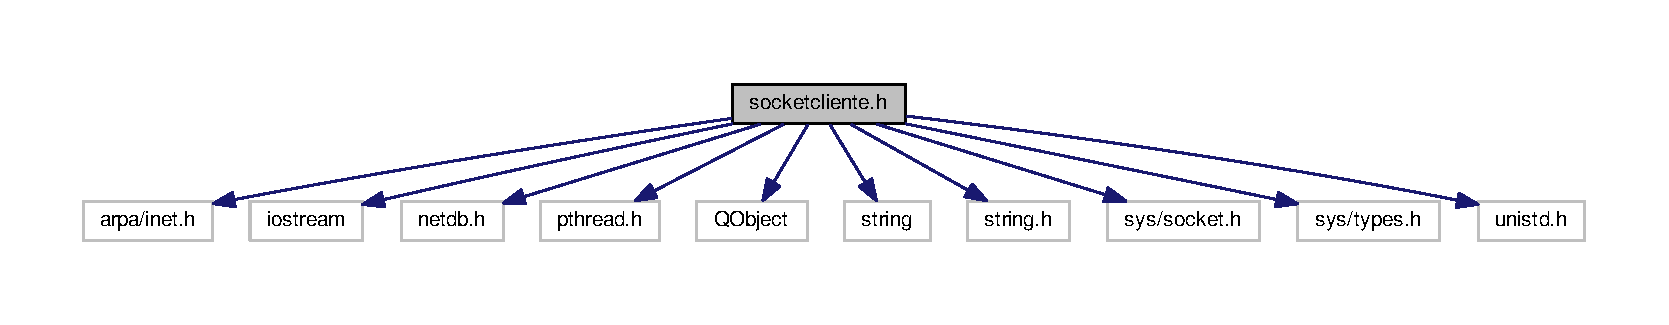
\includegraphics[width=350pt]{socketcliente_8h__incl}
\end{center}
\end{figure}
Gráfico de los archivos que directa o indirectamente incluyen a este archivo\+:
\nopagebreak
\begin{figure}[H]
\begin{center}
\leavevmode
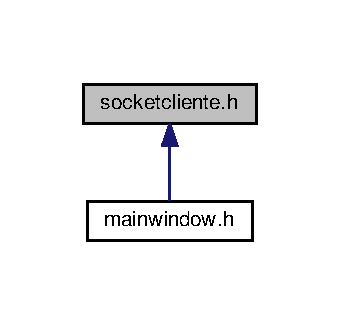
\includegraphics[width=163pt]{socketcliente_8h__dep__incl}
\end{center}
\end{figure}
\subsection*{Clases}
\begin{DoxyCompactItemize}
\item 
class \hyperlink{classSocketCliente}{Socket\+Cliente}
\begin{DoxyCompactList}\small\item\em The \hyperlink{classSocketCliente}{Socket\+Cliente} class. \end{DoxyCompactList}\end{DoxyCompactItemize}


\subsection{Descripción detallada}
Contains a set of methods for handling Socket connection. 

\begin{DoxyAuthor}{Autor}
Erick Andres Obregon Fonseca. 
\end{DoxyAuthor}

%--- End generated contents ---

% Index
\backmatter
\newpage
\phantomsection
\clearemptydoublepage
\addcontentsline{toc}{chapter}{Índice}
\printindex

\end{document}
